\chapter{La Empresa}


\section{Razón Social}
ENGITRONIC S.A.C es una empresa peruana dedicada al desarrollo de sistemas electrónicos y de robótica en el área de automatización, domótica y educación. Además provee servicios de capacitación y venta de equipos electrónicos y de telecomunicaciones. Ver figura ~\ref{fig:logo}.

\begin{figure}[h!]
  \centering
  
\includegraphics[scale=0.2]{images/engitronic.png}
  \caption{Logo de la empresa}
  \label{fig:logo}
\end{figure}

\begin{itemize}
  \item Número de RUC: 20506581983
  \item Razón Social: MECHATRONIC ENGINEERING ENGITRONIC S.A.C
  \item Nombre Comercial: MECHATRONIC
\end{itemize}


\section{Misión, Visión y Objetivos}

\subsection{Misión}
Brindar un servicio de calidad y satisfacción total en el desarrollo de nuevos equipos y prestación de servicios para impulsar las nuevas tecnologías en el país, a través de la mejora continua y la innovación.

\subsection{Visión}
Ser una empresa líder en el desarrollo tecnológico dentro y fuera del país, brindando productos y servicios de alta calidad.

\subsection{Objetivos}
\begin{itemize}
  \item Ofrecer productos de alta innovación tecnológica.
  \item Brindar servicios de calidad en todos nuestros rubros.
  \item Reinventar e innovar en nuestros productos y servicios a fin de estar en la vanguardia tecnológica.
  \item Establecer alianzas estratégicas con diferentes empresas para permitir a los clientes el máximo beneficio posible. 
\end{itemize}


\section{Sobre el Gerente General}
\textbf{Ing. José Oliden Martínez}

Ingeniero Mecatrónico de la Universidad Nacional de Ingeniería (UNI), egreso siendo el primer puesto de su promoción. Director del centro de tecnologías de la información y comunicación CTIC – UNI. Jefe del proyecto Nano satélite Chasqui I – UNI. Presidente del capítulo de la Sociedad de Robótica y Automatización (RAS) de la IEEE Profesor de sistemas embebidos y proyectos de ingeniería en UNI, USMP y UPC. Ex Investigador de la división de Investigación y Desarrollo del INICTEL. Especialización en Robótica aplicada en Japón-México. Especialización en Sistemas Embebidos y RTOS. A través de ENGITRONIC S.A.C ha brindado asesoría, capacitación y soluciones a empresas como: PERUPLAST, Packaging \& Products, MYCOM, UTP, Universidad Católica de Santa María (Arequipa) entre otras empresas nacionales. Como investigador en INICTEL desarrolló actividades como “Diseño e Implementación del sistema TELECARDIO 12”, “CARDIOCELLB138”, Módulos de desarrollo para Microcontroladores, Co diseño e implementación del software CINDA, participación en el proyecto TELETEXTO, ECOGRAFO COMPUTARIZADO y Monitor de latido fetal.


\section{Politica de la empresa o institucion}
La empresa resalta la ética profesional, del trabajo en equipo y la responsabilidad de sus trabajadores, de modo que exista un ambiente de confianza en donde se pueda trabajar de manera óptima. Las responsabilidades delegadas a los trabajadores se orientan a mantener a los trabajadores actualizados con las nuevas tendencias tecnológicas y al desarrollo de sus capacidades de análisis de tecnologías, por ello, siempre la empresa se encuentra en un proceso de investigación continuo. Durante la labor de los practicantes se les hace conocer el funcionamiento de los diversos equipos dentro de la empresa con la intención de que los practicantes puedan usarlos y así apoyar a su proceso de aprendizaje. La empresa muestra interés por la identificación personal con la empresa, así como el bienestar personal de cada uno de sus trabajadores, por tal motivo realiza charlas y reuniones por eventos importantes.


\section{Productos y Servicios de la Empresa}

\subsection{Diseño y fabricación de sistemas embebidos}
\begin{itemize}
  \item Módulos de desarrollo y grabación para microcontroladores Freescale y Microchip. Ver figuras ~\ref{fig:modulo-programador-pic} y ~\ref{fig:modulo-programador-motorola}.
    \begin{figure}[h!]
      \centering
      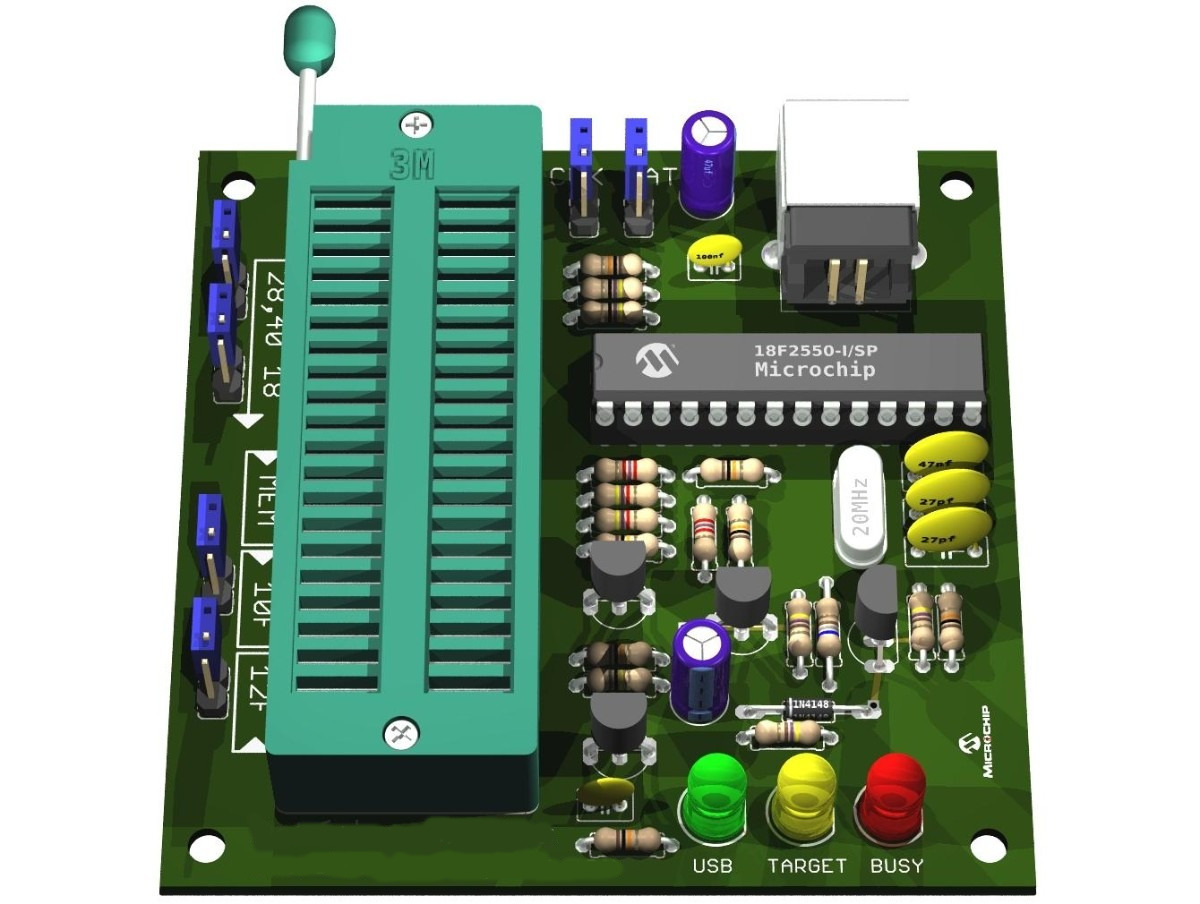
\includegraphics[scale=0.2]{images/company/modulo-programador-pic.jpg}
      \caption{Módulo Programador PIC}
      \label{fig:modulo-programador-pic}
    \end{figure}
    \begin{figure}[h!]
      \centering
      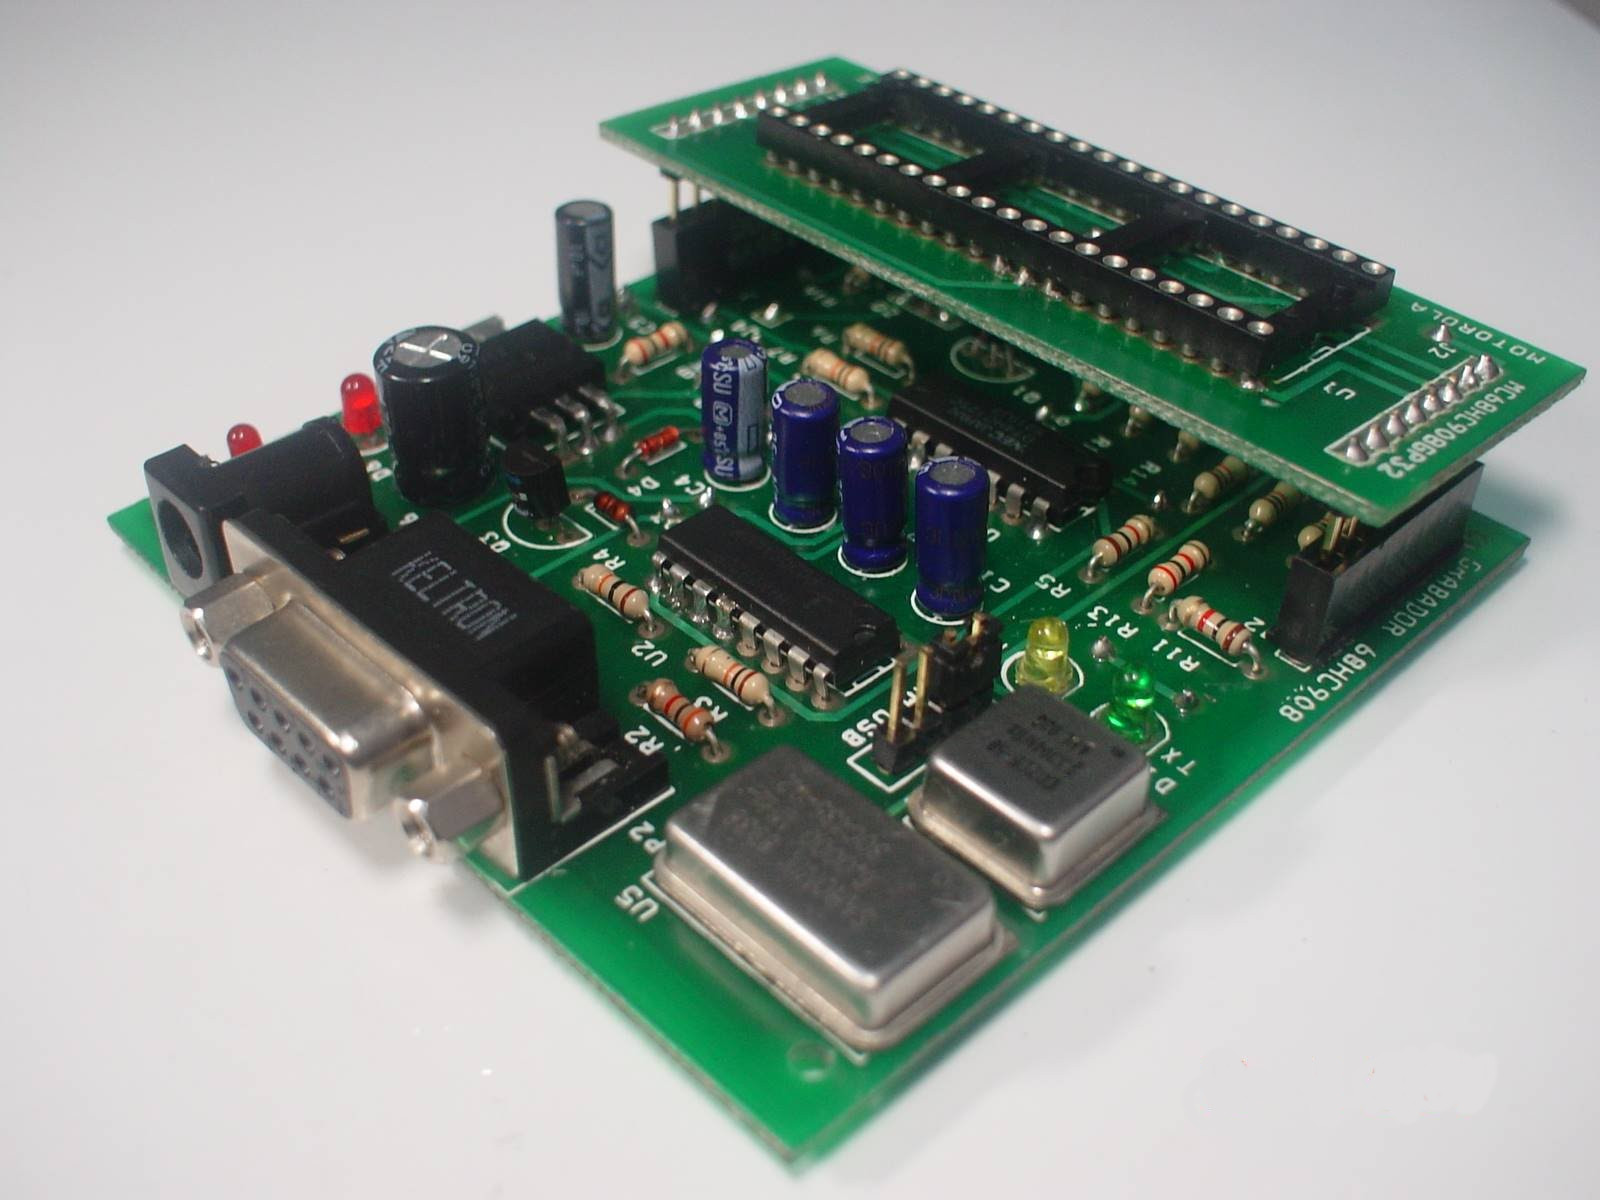
\includegraphics[scale=0.15]{images/company/modulo-programador-motorola.jpg}
      \caption{Módulo Programador Motorola}
      \label{fig:modulo-programador-motorola}
    \end{figure}
  \item Módulo entrenador para microcontroladores. Ver figura ~\ref{fig:entrenador-pic}.
    \begin{figure}[h!]
      \centering
      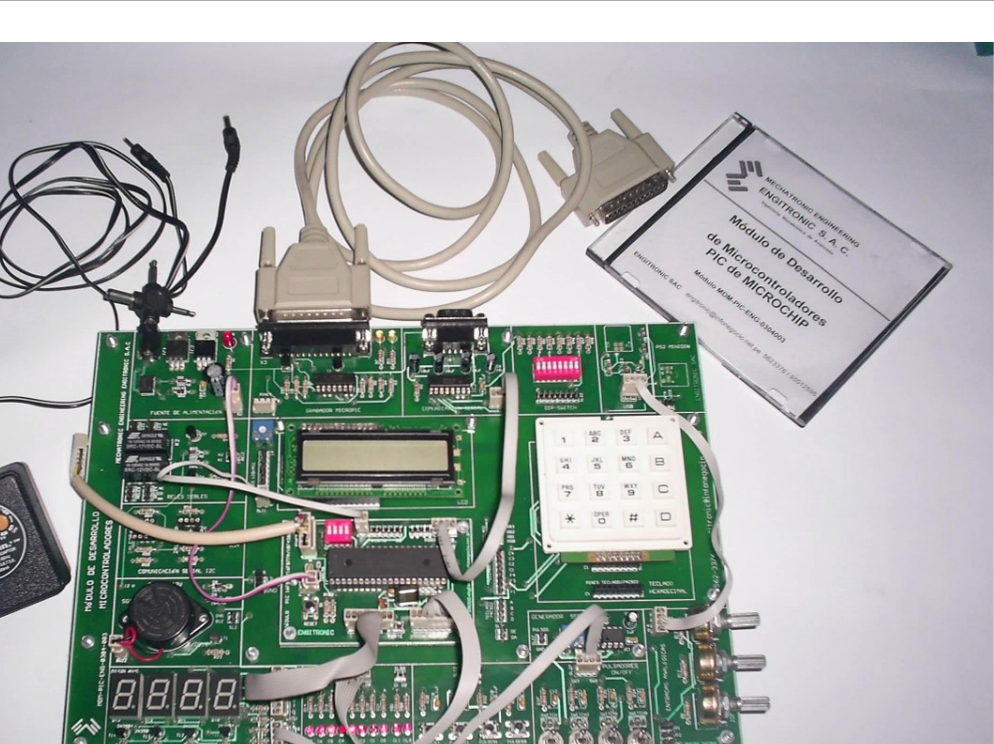
\includegraphics[scale=0.2]{images/company/entrenador-pic.png}
      \caption{Módulo entrenador para microcontroladores}
      \label{fig:entrenador-pic}
    \end{figure}
  \item Circuitos de telecomunicaciones. Ver figura ~\ref{fig:modulo-gps}. 
    \begin{figure}[h!]
      \centering
      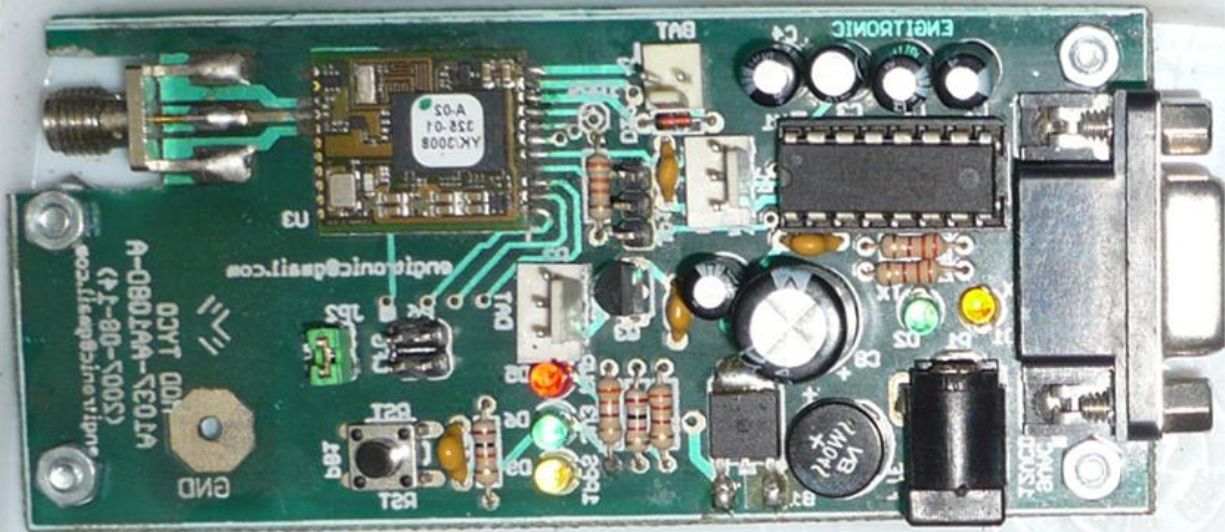
\includegraphics[scale=0.2]{images/company/modulo-gps.png}
      \caption{Módulo GPS 1080}
      \label{fig:modulo-gps}
    \end{figure}
\end{itemize}

\subsection{Implementación de sistemas para automatización}
Módulos de entrenamiento para PLCs. Ver figura ~\ref{fig:modulo-plc}. 
\begin{figure}[h!]
  \centering
  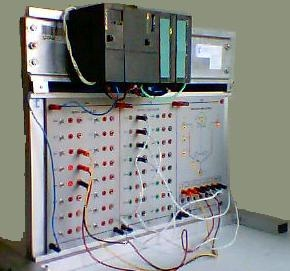
\includegraphics[scale=0.8]{images/company/modulo-plc.jpg}
  \caption{PLC Siemens}
  \label{fig:modulo-plc}
\end{figure}

\subsection{Diseño e implementación de sistemas robóticos}
\begin{itemize}
  \item Manipuladores Robóticos de propósito educativo.
  \item Robots seguidores de línea.
  \item Robots seguidores de luz.
  \item Robots móviles telecontrolados.
\end{itemize}

\subsection{Capacitaciones}
\begin{itemize}
  \item Curso de capacitación en programación de sistemas embebidos. Ver figura ~\ref{fig:capacitaciones}.
    \begin{figure}[h!]
      \centering
      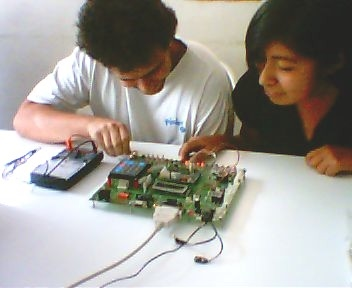
\includegraphics[scale=0.5]{images/company/capacitaciones.jpg}
      \caption{Capacitación en sistemas embebidos}
      \label{fig:capacitaciones}
    \end{figure}
  \item Visual C\# para aplicaciones con microcontroladores.
  \item C para microcontroladores PIC.
  \item C para microcontroladores MOTOROLA, Aplicaciones en Robótica y
  Radiofrecuencia.
  \item Introducción a la robótica.
  \item Automatización Industrial.
\end{itemize}

\subsection{Venta de equipos electrónicos y de telecomunicaciones}
\begin{itemize}
  \item Antenas GPRS.
  \item Módulos de desarrollo para microcontroladores.
  \item Circuitos electrónicos.
  \item Exportación de software especializado.
\end{itemize}


\section{Localización}

El domicilio fiscal de la empresa es Calle Luis Romero Nro. 1025 Urb. Roma (Altura Cdra. 26 Av. Oscar R. Benavides) Lima-Lima. Referencia: Cruce de la Ex. Av. Colonial y la Av. Universitaria. Ver figura ~\ref{fig:location}.

\begin{figure}[h!]
  \centering
  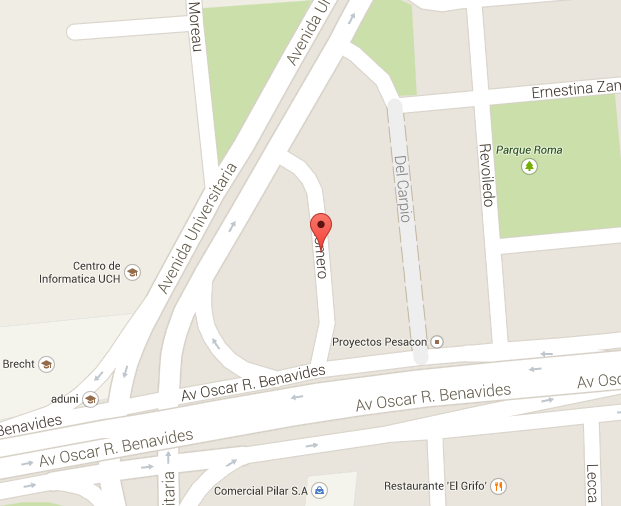
\includegraphics[scale=0.5]{images/location.png}
  \caption{Ubicación de la Empresa}
  \label{fig:location}
\end{figure}


\section{Infraestructura Productiva}

Las instalaciones de la empresa cuentan con un Almacén, un área de mecánica, un área de electrónica, un área de desarrollo de proyectos y una nueva área de cómputo implementada durante la práctica.

Los equipos disponibles en la empresa son:

\begin{itemize}
  \item Taladro de mesa. Ver figura ~\ref{fig:taladro-mesa}.
    \begin{figure}[h!]
      \centering
      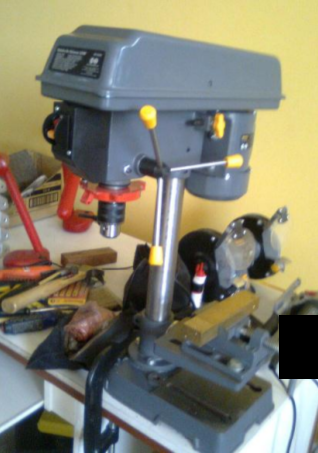
\includegraphics[scale=0.5]{images/company/taladro-mesa.png}
      \caption{Taladro de mesa}
      \label{fig:taladro-mesa}
    \end{figure}
  \item Esmeril. Ver figura ~\ref{fig:esmeril}.
    \begin{figure}[h!]
      \centering
      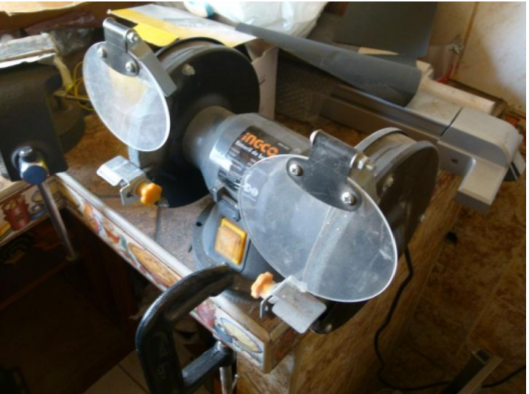
\includegraphics[scale=0.5]{images/company/esmeril.png}
      \caption{Esmeril}
      \label{fig:esmeril}
    \end{figure}
  \item Sierra Eléctrica. Ver figura ~\ref{fig:sierra-electrica}.
    \begin{figure}[h!]
      \centering
      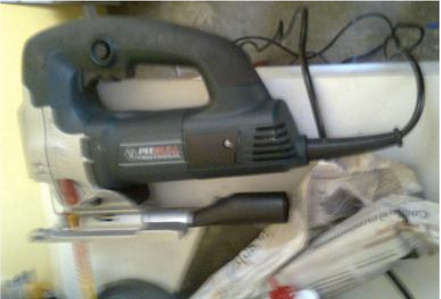
\includegraphics[scale=0.5]{images/company/sierra-electrica.png}
      \caption{Sierra Eléctrica}
      \label{fig:sierra-electrica}
    \end{figure}
  \item Prensa de banco. Ver figura ~\ref{fig:prensa-banco}.
    \begin{figure}[h!]
      \centering
      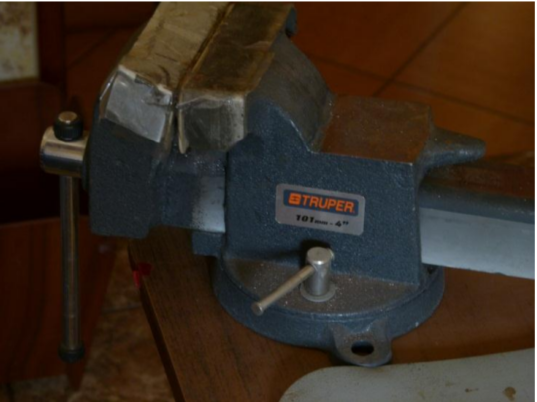
\includegraphics[scale=0.5]{images/company/prensa-banco.png}
      \caption{Prensa de banco}
      \label{fig:prensa-banco}
    \end{figure}
  \item Caja de circuitería electrónica. Ver figura ~\ref{fig:componentes-electronicos}.
    \begin{figure}[h!]
      \centering
      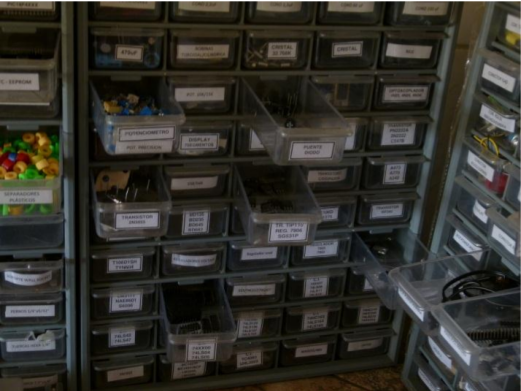
\includegraphics[scale=0.5]{images/company/componentes-electronicos.png}
      \caption{Componentes electrónicos y varios}
      \label{fig:componentes-electronicos}
    \end{figure}
\end{itemize}